\section{Gaussian Distributions}

The behaviour of all quantitative traits of the dataset is assumed to adhere to a
Gaussian Distribution.
This assumption is taken due to how the values of the data set are presented.
As shown in Figures
% \ref{fig: sepal length normal distribution},
% \ref{fig: sepal width normal distribution},
\ref{fig: petal length normal distribution} and
\ref{fig: petal width normal distribution}
the distribution for each flower variety follows the
general behaviour of the Gaussian Distribution.

Having confirmed that all quantitative features of the dataset
adhere to Gaussian Distributions, it is possible to proceed with the
development of the classifiers.

% \begin{figure}[htb!]
%  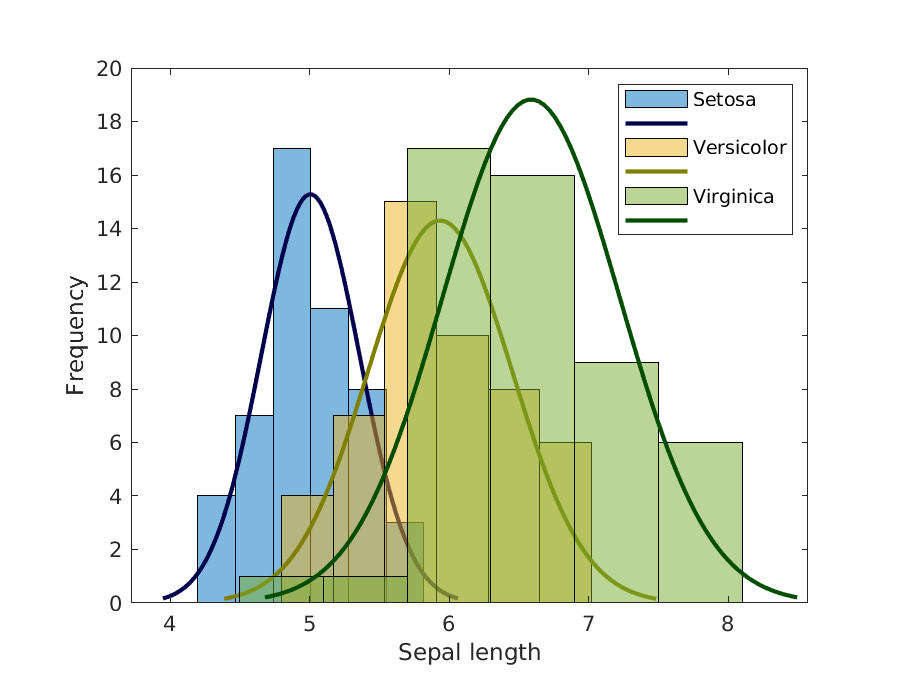
\includegraphics[width=\textwidth]{normSepalLength}
%  \caption{Sepal Length}
%  \label{fig: sepal length normal distribution}
% \end{figure}
%
% \begin{figure}[htb!]
%  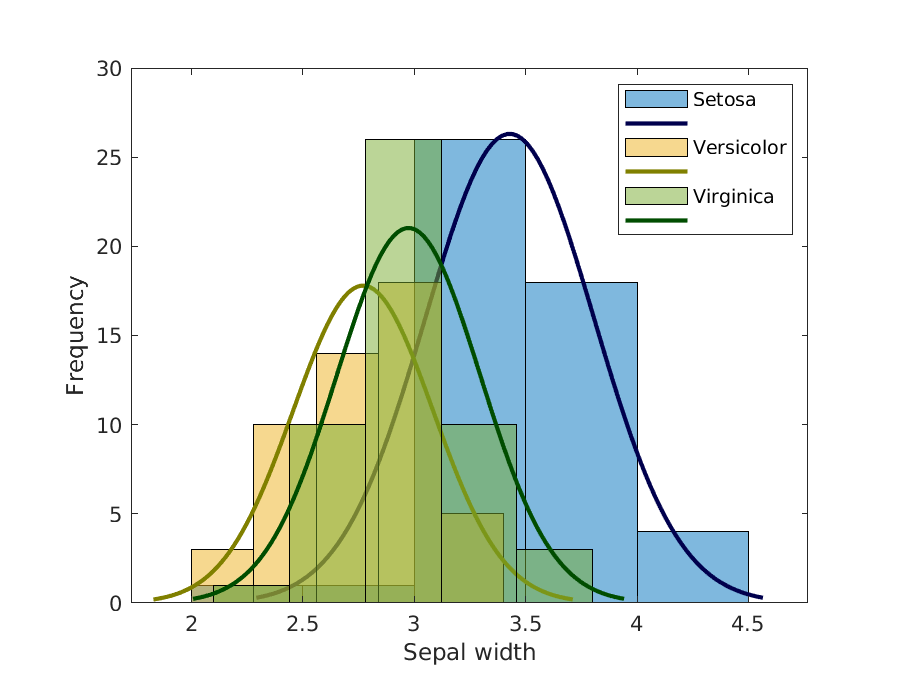
\includegraphics[width=\textwidth]{normSepalWidth}
%  \caption{Sepal Width}
%  \label{fig: sepal width normal distribution}
% \end{figure}

\begin{figure}[htb!]
 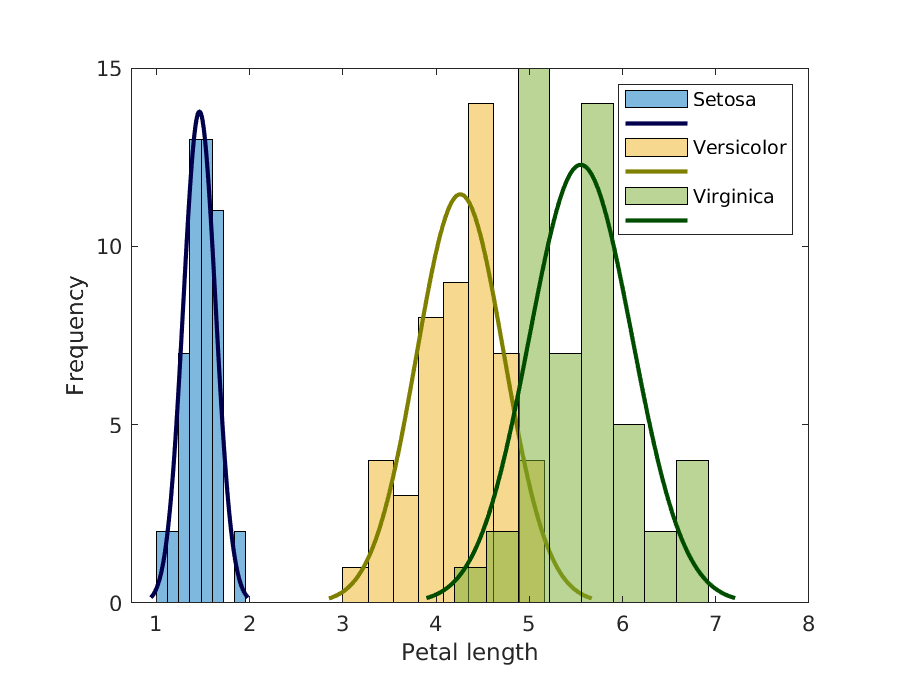
\includegraphics[width=\textwidth]{normPetalLength}
 \caption{Petal Length}
 \label{fig: petal length normal distribution}
\end{figure}

\begin{figure}[htb!]
 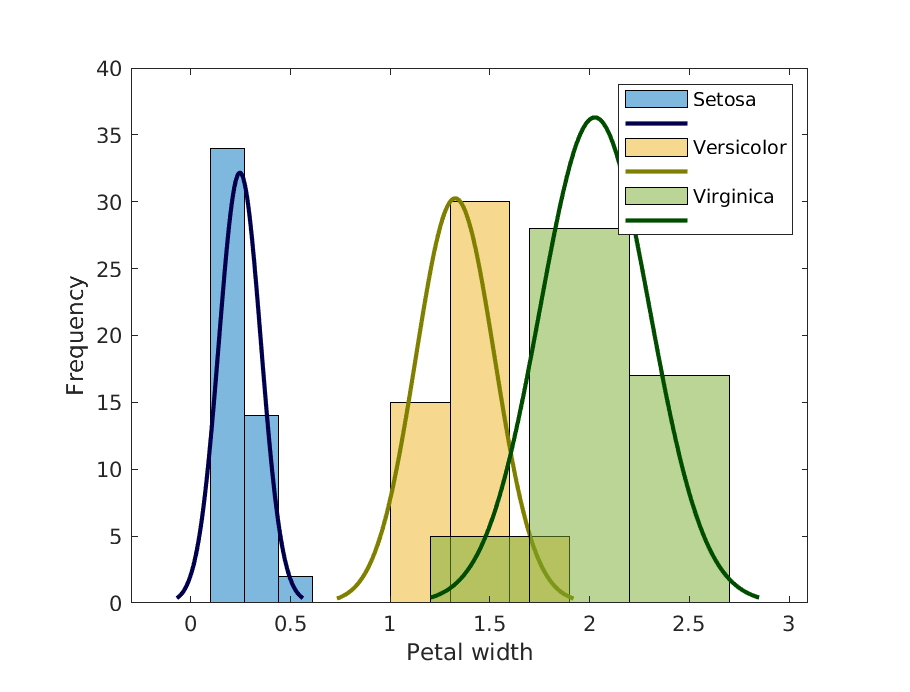
\includegraphics[width=\textwidth]{normPetalWidth}
 \caption{Petal Width}
 \label{fig: petal width normal distribution}
\end{figure}



\pagebreak
\newpage
